\documentclass[12pt,a4paper]{article}
\usepackage{lmodern}

\usepackage{placeins}
\usepackage{amssymb,amsmath}
\usepackage{ifxetex,ifluatex}
\usepackage{fixltx2e} % provides \textsubscript
\ifnum 0\ifxetex 1\fi\ifluatex 1\fi=0 % if pdftex
  \usepackage[T1]{fontenc}
  \usepackage[utf8]{inputenc}
\else % if luatex or xelatex
  \ifxetex
    \usepackage{mathspec}
    \usepackage{xltxtra,xunicode}
  \else
    \usepackage{fontspec}
  \fi
  \defaultfontfeatures{Mapping=tex-text,Scale=MatchLowercase}
  \newcommand{\euro}{€}
\fi
% use upquote if available, for straight quotes in verbatim environments
\IfFileExists{upquote.sty}{\usepackage{upquote}}{}
% use microtype if available
\IfFileExists{microtype.sty}{%
\usepackage{microtype}
\UseMicrotypeSet[protrusion]{basicmath} % disable protrusion for tt fonts
}{}
\usepackage[lmargin = 2cm, rmargin = 2cm, tmargin = 2cm, bmargin = 2.5cm]{geometry}


% Figure Placement:
\usepackage{float}
\let\origfigure\figure
\let\endorigfigure\endfigure
\renewenvironment{figure}[1][2] {
    \expandafter\origfigure\expandafter[H]
} {
    \endorigfigure
}

%%%% Jens %%%%
\usepackage{titlesec}
\DeclareMathOperator*{\argmax}{arg\,max}
\DeclareMathOperator*{\argmin}{arg\,min}
\renewcommand{\vec}{\operatorname{vec}}
\newcommand{\tr}{\operatorname{tr}}
\newcommand{\Var}{\operatorname{Var}} % Variance
\newcommand{\VAR}{\operatorname{VAR}} % Vector autoregression
\newcommand{\Lag}{\operatorname{L}} % Lag operator
\newcommand{\Cov}{\operatorname{Cov}}
\newcommand{\diag}{\operatorname{diag}}
\newcommand{\adj}{\operatorname{adj}}
\newcommand{\loglik}{\operatorname{ll}}

\allowdisplaybreaks

\titleformat{\section}
{\normalfont\large\bfseries}{\thesection}{1em}{}

\newcommand{\tmpsection}[1]{}
\let\tmpsection=\section
\renewcommand{\section}[1]{\tmpsection{\underline{#1}} }





%% citation setup
\usepackage{csquotes}

\usepackage[backend=biber, maxbibnames = 99, style = apa]{biblatex}
\setlength\bibitemsep{1.5\itemsep}
\addbibresource{R_packages.bib}
\usepackage{color}
\usepackage{fancyvrb}
\newcommand{\VerbBar}{|}
\newcommand{\VERB}{\Verb[commandchars=\\\{\}]}
\DefineVerbatimEnvironment{Highlighting}{Verbatim}{commandchars=\\\{\}}
% Add ',fontsize=\small' for more characters per line
\usepackage{framed}
\definecolor{shadecolor}{RGB}{248,248,248}
\newenvironment{Shaded}{\begin{snugshade}}{\end{snugshade}}
\newcommand{\AlertTok}[1]{\textcolor[rgb]{0.94,0.16,0.16}{#1}}
\newcommand{\AnnotationTok}[1]{\textcolor[rgb]{0.56,0.35,0.01}{\textbf{\textit{#1}}}}
\newcommand{\AttributeTok}[1]{\textcolor[rgb]{0.77,0.63,0.00}{#1}}
\newcommand{\BaseNTok}[1]{\textcolor[rgb]{0.00,0.00,0.81}{#1}}
\newcommand{\BuiltInTok}[1]{#1}
\newcommand{\CharTok}[1]{\textcolor[rgb]{0.31,0.60,0.02}{#1}}
\newcommand{\CommentTok}[1]{\textcolor[rgb]{0.56,0.35,0.01}{\textit{#1}}}
\newcommand{\CommentVarTok}[1]{\textcolor[rgb]{0.56,0.35,0.01}{\textbf{\textit{#1}}}}
\newcommand{\ConstantTok}[1]{\textcolor[rgb]{0.00,0.00,0.00}{#1}}
\newcommand{\ControlFlowTok}[1]{\textcolor[rgb]{0.13,0.29,0.53}{\textbf{#1}}}
\newcommand{\DataTypeTok}[1]{\textcolor[rgb]{0.13,0.29,0.53}{#1}}
\newcommand{\DecValTok}[1]{\textcolor[rgb]{0.00,0.00,0.81}{#1}}
\newcommand{\DocumentationTok}[1]{\textcolor[rgb]{0.56,0.35,0.01}{\textbf{\textit{#1}}}}
\newcommand{\ErrorTok}[1]{\textcolor[rgb]{0.64,0.00,0.00}{\textbf{#1}}}
\newcommand{\ExtensionTok}[1]{#1}
\newcommand{\FloatTok}[1]{\textcolor[rgb]{0.00,0.00,0.81}{#1}}
\newcommand{\FunctionTok}[1]{\textcolor[rgb]{0.00,0.00,0.00}{#1}}
\newcommand{\ImportTok}[1]{#1}
\newcommand{\InformationTok}[1]{\textcolor[rgb]{0.56,0.35,0.01}{\textbf{\textit{#1}}}}
\newcommand{\KeywordTok}[1]{\textcolor[rgb]{0.13,0.29,0.53}{\textbf{#1}}}
\newcommand{\NormalTok}[1]{#1}
\newcommand{\OperatorTok}[1]{\textcolor[rgb]{0.81,0.36,0.00}{\textbf{#1}}}
\newcommand{\OtherTok}[1]{\textcolor[rgb]{0.56,0.35,0.01}{#1}}
\newcommand{\PreprocessorTok}[1]{\textcolor[rgb]{0.56,0.35,0.01}{\textit{#1}}}
\newcommand{\RegionMarkerTok}[1]{#1}
\newcommand{\SpecialCharTok}[1]{\textcolor[rgb]{0.00,0.00,0.00}{#1}}
\newcommand{\SpecialStringTok}[1]{\textcolor[rgb]{0.31,0.60,0.02}{#1}}
\newcommand{\StringTok}[1]{\textcolor[rgb]{0.31,0.60,0.02}{#1}}
\newcommand{\VariableTok}[1]{\textcolor[rgb]{0.00,0.00,0.00}{#1}}
\newcommand{\VerbatimStringTok}[1]{\textcolor[rgb]{0.31,0.60,0.02}{#1}}
\newcommand{\WarningTok}[1]{\textcolor[rgb]{0.56,0.35,0.01}{\textbf{\textit{#1}}}}
\usepackage{graphicx}
\makeatletter
\def\maxwidth{\ifdim\Gin@nat@width>\linewidth\linewidth\else\Gin@nat@width\fi}
\def\maxheight{\ifdim\Gin@nat@height>\textheight\textheight\else\Gin@nat@height\fi}
\makeatother
% Scale images if necessary, so that they will not overflow the page
% margins by default, and it is still possible to overwrite the defaults
% using explicit options in \includegraphics[width, height, ...]{}
\setkeys{Gin}{width=\maxwidth,height=\maxheight,keepaspectratio}
\ifxetex
  \usepackage[setpagesize=false, % page size defined by xetex
              unicode=false, % unicode breaks when used with xetex
              xetex]{hyperref}
\else
  \usepackage[unicode=true, linktocpage = TRUE]{hyperref}
\fi
\hypersetup{breaklinks=true,
            bookmarks=true,
            pdfauthor={Dr.~Yannick Hoga},
            pdftitle={Multivariate Time Series Analysis},
            colorlinks=true,
            citecolor=black,
            urlcolor=black,
            linkcolor=black,
            pdfborder={0 0 0}}
\urlstyle{same}  % don't use monospace font for urls
\setlength{\parindent}{0pt}
\setlength{\parskip}{6pt plus 2pt minus 1pt}
\setlength{\emergencystretch}{3em}  % prevent overfull lines
\setcounter{secnumdepth}{5}

%%% Use protect on footnotes to avoid problems with footnotes in titles
\let\rmarkdownfootnote\footnote%
\def\footnote{\protect\rmarkdownfootnote}

%%% Change title format to be more compact
\usepackage{titling}

% Create subtitle command for use in maketitle
\newcommand{\subtitle}[1]{
  \posttitle{
    \begin{center}\large#1\end{center}
    }
}

\setlength{\droptitle}{-2em}
  \title{Multivariate Time Series Analysis}
  \pretitle{\vspace{\droptitle}\centering\huge}
  \posttitle{\par}
\subtitle{Solution Exercise Sheet 4}
  \author{Dr.~Yannick Hoga}
  \preauthor{\centering\large\emph}
  \postauthor{\par}
  \date{}
  \predate{}\postdate{}


%% linespread settings

\usepackage{setspace}

\onehalfspacing


% Language Setup

\usepackage{ifthen}
\usepackage{iflang}
\usepackage[super]{nth}
\usepackage[ngerman, english]{babel}

%Acronyms
\usepackage[printonlyused, withpage, nohyperlinks]{acronym}
\usepackage{changepage}

% Multicols for the Title page
\usepackage{multicol}


% foot


\begin{document}

\selectlanguage{english}

%%%%%%%%%%%%%% Jens %%%%%
\numberwithin{equation}{section}




\restoregeometry


%%% Header 

\begin{minipage}{0.6\textwidth}
University of Duisburg-Essen\\
Faculty of Business Administration and Economics\\
Chair of Econometrics\\
\end{minipage}

%\begin{minipage}{0.4\textwidth}
	\begin{flushright}
	\vspace{-3cm}
	\includegraphics*[width=5cm]{../Includes/duelogo_en.png}\\
	\vspace{.125cm}
	\end{flushright}
%\end{minipage}
%\vspace{.125cm}
\hspace{-0.005cm}Winter Term 2019/2020

\vspace{0.05cm}

\begin{center}
	\vspace{.25cm}
	Dr.~Yannick Hoga \hspace{.5cm} Thilo Reinschlüssel \\
	\vspace{.25cm}
	\textbf{\Large{Multivariate Time Series Analysis}}\\
	\vspace{.25cm}
	\textbf{\large{Solution Exercise Sheet 4}}\\
	\vspace{.125cm}
\end{center}




% body from markdown

\hypertarget{exercise-1-implied-models-for-components}{%
\section{Exercise 1: Implied Models for
Components}\label{exercise-1-implied-models-for-components}}

Consider the VAR(1) model \(z_t = \phi_0 + \phi_1 z_{t-1} + a_t\) from
the Exercise Sheet 3 again:

\begin{align*}
    \phi_0 = \begin{pmatrix} 1 \\ 0 \end{pmatrix}, \quad \phi_1 = \begin{pmatrix} 0.75 & 0 \\ -0.25 & 0.5 \end{pmatrix}, \quad \Sigma_a = \begin{pmatrix} 1 & 0 \\ 0 & 1 \end{pmatrix} \ \text{.}
\end{align*}

\begin{itemize}
    \item[a)] Write down the model using lag operator notation. Then rearrange the equation such that
all parts based on $z_t$ are on the left-hand side and the remainder is on the right-hand side. 
\end{itemize}

\emph{Solution:}

\begin{align*}
  \text{Model:} z_t & = \phi_0 + \phi_1 z_{t-1} + a_t\\  
  \text{Lag notation:} \ z_t & = \phi_0 + \phi_1 \Lag z_t + a_t\\
  \\
  \Leftrightarrow z_t - \phi_1 \Lag Z_t & = \phi_0 + a_t
\end{align*}

\begin{itemize}
    \item[b)] By factoring out $z_t$ on the left, we obtain the lag polynomial $\phi (\Lag)$. Compute its adjoint matrix by hand.
    \item[]  \textit{Hint: Treat the lag operator as some scalar. The adjoint matrix can be computed like the inverse matrix but \textbf{without} the scaling by}  $\dfrac{1}{\det (\phi (\Lag))} \text{.}$
\end{itemize}

\emph{Solution:}

\begin{align*}
  \underbrace{\left( I - \phi_1 \Lag \right)}_{=: \phi \Lag} z_t & = \phi_0 + a_t\\
  \Leftrightarrow \phi (\Lag) & = \begin{pmatrix} 1- 0.75 \Lag & 0 \\ -0.25 \Lag & 1 - 0.5 \Lag  \end{pmatrix}\\
  \Leftrightarrow  \phi^{\adj} & = \begin{pmatrix} 1- 0.5 \Lag & 0 \\ 0.25 \Lag & 1 - 0.75 \Lag  \end{pmatrix}\\
\end{align*}

\begin{itemize}
    \item[c)]Pre-multiply the model equation you got in part a) with the adjoint matrix you computed in part b).
    \item[]  \textit{Hint: You are supposed to end up with a diagonal matrix.}
\end{itemize}

\emph{Solution:}

\begin{tiny}
\begin{align*}
  \begin{pmatrix} 1- 0.5 \Lag & 0 \\ 0.25 \Lag & 1 - 0.75 \Lag  \end{pmatrix} \begin{pmatrix} 1- 0.75 \Lag & 0 \\ -0.25 \Lag & 1 - 0.5 \Lag  \end{pmatrix} z_t & = \begin{pmatrix} 1 - 0.75 \Lag & 0 \\ 0.25 \Lag & 1 - 0.75 \Lag \end{pmatrix} \cdot \left( \phi_0 + a_t \right) \\
  \Leftrightarrow \begin{pmatrix} (1- 0.5 \Lag) (1- 0.75 \Lag) & 0 \\
  (0.25 \Lag) (1 - 0.75 \Lag) + (1 - 0.75 \Lag) (-0.25 \Lag) & (1 - 0.75 \Lag) (1 - 0.5 \Lag)
  \end{pmatrix} z_t  & = 
  \begin{pmatrix} (1 - 0.5 \Lag) \cdot 1 \\ 0.25 \Lag \cdot 1 +(1- 0.75 \Lag) \cdot 0 \end{pmatrix} +  
  \begin{pmatrix} (1 - 0.5 \Lag) \cdot a_{1,t} \\ (0.25 \Lag ) a_{1,t} + 1 (1- 0.75 \Lag) a_{2,t}\end{pmatrix} \\
  \Leftrightarrow \begin{pmatrix} z_{1,t} - 1.25 z_{1, t-1} + 0.375 z_{1, t-2} \\ z_{2,t} - 1.25 z_{2, t-1} + 0.375 z_{2, t-2} \end{pmatrix} 
  & = \begin{pmatrix} 0.5 \\ 0.25 \end{pmatrix} + \begin{pmatrix} a_{1,t} - 0.5 a_{1, t-1} \\ 
  0 + 0.25 a_{1, t-1} + a_{2,t} - 0.75 a_{2, t-1}\end{pmatrix}  
\end{align*}
\end{tiny}

\begin{itemize}
    \item[d)] The result of part c) should be a collection of two univariate ARMA(p,q) models. What is the lag order of both models?
\end{itemize}

\emph{Solution:}

The lag order of both models is ARMA(2,1)

\begin{itemize}
    \item[e)] Simulate a trajectory with T = 1000 of the original VAR(1) model.
    \item[]  \textit{Hint:’VARMAsim’ on Slide 2–6.}
\end{itemize}

\emph{Solution:}

\begin{Shaded}
\begin{Highlighting}[]
\CommentTok{# Preparation: Define matrices}
\NormalTok{phi_}\DecValTok{1}\NormalTok{ <-}\StringTok{ }\KeywordTok{matrix}\NormalTok{(}\DataTypeTok{data =} \KeywordTok{c}\NormalTok{(}\FloatTok{0.75}\NormalTok{, }\FloatTok{-0.25}\NormalTok{, }\DecValTok{0}\NormalTok{, }\FloatTok{0.5}\NormalTok{), }\DataTypeTok{nrow =} \DecValTok{2}\NormalTok{)}
\NormalTok{phi_}\DecValTok{0}\NormalTok{ <-}\StringTok{ }\KeywordTok{c}\NormalTok{(}\DecValTok{1}\NormalTok{, }\DecValTok{0}\NormalTok{)}
\NormalTok{Sigma_a <-}\StringTok{ }\KeywordTok{matrix}\NormalTok{(}\DataTypeTok{data =} \KeywordTok{c}\NormalTok{(}\DecValTok{1}\NormalTok{, }\DecValTok{0}\NormalTok{, }\DecValTok{0}\NormalTok{, }\DecValTok{1}\NormalTok{), }\DataTypeTok{nrow =} \DecValTok{2}\NormalTok{)}

\NormalTok{N <-}\StringTok{ }\DecValTok{10}\OperatorTok{^}\DecValTok{3} \CommentTok{# length of trajectory }
\NormalTok{burn_in <-}\StringTok{ }\DecValTok{250} \CommentTok{# extra periods, are then cut away from the simulated}
\CommentTok{#to reduce the impact of starting point selection}

\KeywordTok{set.seed}\NormalTok{(}\DecValTok{42}\NormalTok{) }\CommentTok{# set seed for reproducibility}

\NormalTok{var1_data <-}\StringTok{ }\KeywordTok{VARMAsim}\NormalTok{(}\DataTypeTok{nobs =}\NormalTok{ N, }\DataTypeTok{arlags =} \KeywordTok{c}\NormalTok{(}\DecValTok{1}\NormalTok{), }\DataTypeTok{malags =} \OtherTok{NULL}\NormalTok{, }
                      \DataTypeTok{cnst =}\NormalTok{ phi_}\DecValTok{0}\NormalTok{, }\DataTypeTok{phi =}\NormalTok{ phi_}\DecValTok{1}\NormalTok{, }\DataTypeTok{skip =}\NormalTok{ burn_in, }\DataTypeTok{sigma =}\NormalTok{ Sigma_a)}

\KeywordTok{plot.ts}\NormalTok{(var1_data}\OperatorTok{$}\NormalTok{series)}
\end{Highlighting}
\end{Shaded}

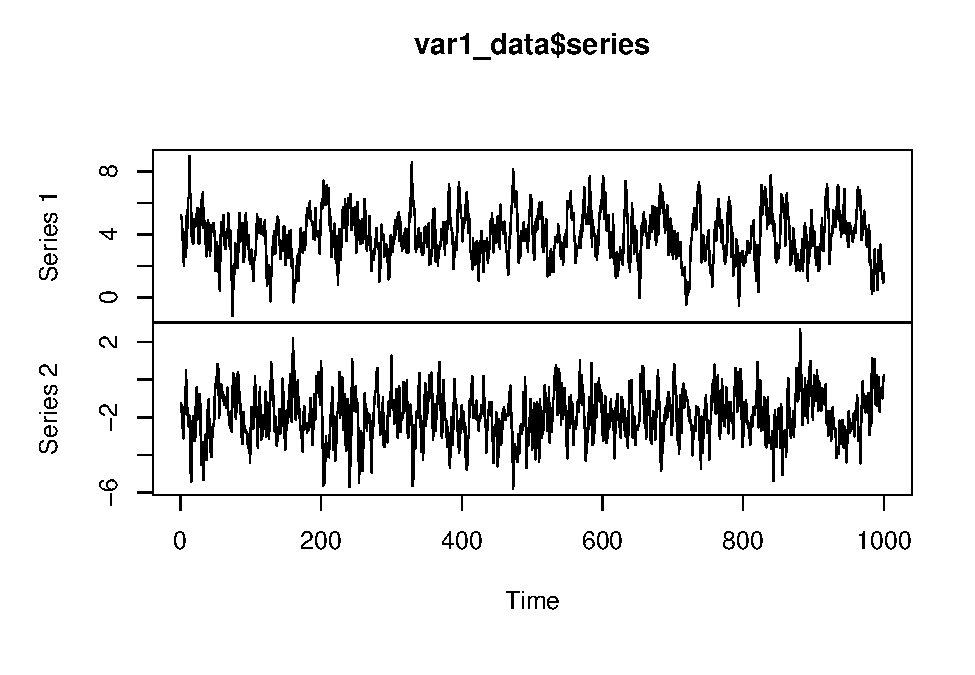
\includegraphics{solution_exercise_4_files/figure-latex/1_e-1.pdf}

\begin{itemize}
    \item[f)] Fit a VAR(1) model to the data, store the results as a variable and estimate the predictions’ mean squared error for each variable in $z_t$
\end{itemize}

\emph{Solution:}

\begin{Shaded}
\begin{Highlighting}[]
\NormalTok{var1_fit <-}\StringTok{ }\KeywordTok{VAR}\NormalTok{(}\DataTypeTok{x =}\NormalTok{ var1_data}\OperatorTok{$}\NormalTok{series, }\DataTypeTok{p =} \KeywordTok{c}\NormalTok{(}\DecValTok{1}\NormalTok{), }\DataTypeTok{include.mean =} \OtherTok{TRUE}\NormalTok{) }
\end{Highlighting}
\end{Shaded}

\begin{verbatim}
## Constant term: 
## Estimates:  0.9776701 -0.03392965 
## Std.Error:  0.09103255 0.08841188 
## AR coefficient matrix 
## AR( 1 )-matrix 
##        [,1]     [,2]
## [1,]  0.747 -0.00125
## [2,] -0.226  0.51979
## standard error 
##        [,1]   [,2]
## [1,] 0.0222 0.0260
## [2,] 0.0215 0.0253
##   
## Residuals cov-mtx: 
##            [,1]       [,2]
## [1,] 1.02729516 0.01620576
## [2,] 0.01620576 0.96899845
##   
## det(SSE) =  0.9951848 
## AIC =  0.003173153 
## BIC =  0.02280417 
## HQ  =  0.01063431
\end{verbatim}

\begin{Shaded}
\begin{Highlighting}[]
\NormalTok{mse_var <-}\StringTok{ }\KeywordTok{colMeans}\NormalTok{(var1_fit}\OperatorTok{$}\NormalTok{residuals}\OperatorTok{^}\DecValTok{2}\NormalTok{) }\CommentTok{# MSEs of two sequences of residuals (a_1, a_2)}
\NormalTok{mse_var}
\end{Highlighting}
\end{Shaded}

\begin{verbatim}
## [1] 1.0272952 0.9689984
\end{verbatim}

As we can see the estimation of a VAR(1) comes pretty close to the
\enquote{true} (simulated) values of \(\phi_0\) and \(\phi_1\)

\begin{Shaded}
\begin{Highlighting}[]
\NormalTok{mse_var <-}\StringTok{ }\KeywordTok{colMeans}\NormalTok{(var1_fit}\OperatorTok{$}\NormalTok{residuals}\OperatorTok{^}\DecValTok{2}\NormalTok{) }\CommentTok{# MSEs of two sequences of residuals}
\NormalTok{mse_var}
\end{Highlighting}
\end{Shaded}

\begin{verbatim}
## [1] 1.0272952 0.9689984
\end{verbatim}

The MSEs are as we would expected, given \(\Sigma_a\).

\begin{itemize}
    \item[g)] Repeat the task by fitting the two ARMA(p,q) models from b) to the data. Again compute the mean squared error for $z_{1,t}$ and $z_{2,t}$ each.
    \item[]  \textit{Hint:’arima’.}
\end{itemize}

\emph{Solution:}

\begin{Shaded}
\begin{Highlighting}[]
\NormalTok{z1_fit <-}\StringTok{ }\KeywordTok{arima}\NormalTok{(}\DataTypeTok{x =}\NormalTok{ var1_data}\OperatorTok{$}\NormalTok{series[,}\DecValTok{1}\NormalTok{], }\DataTypeTok{order =} \KeywordTok{c}\NormalTok{(}\DecValTok{2}\NormalTok{,}\DecValTok{0}\NormalTok{,}\DecValTok{1}\NormalTok{), }\DataTypeTok{include.mean =} \OtherTok{TRUE}\NormalTok{)}
\NormalTok{z2_fit <-}\StringTok{ }\KeywordTok{arima}\NormalTok{(}\DataTypeTok{x =}\NormalTok{ var1_data}\OperatorTok{$}\NormalTok{series[,}\DecValTok{2}\NormalTok{], }\DataTypeTok{order =} \KeywordTok{c}\NormalTok{(}\DecValTok{2}\NormalTok{,}\DecValTok{0}\NormalTok{,}\DecValTok{1}\NormalTok{), }\DataTypeTok{include.mean =} \OtherTok{TRUE}\NormalTok{, }
                \DataTypeTok{optim.control =} \KeywordTok{list}\NormalTok{(}\DataTypeTok{maxit =} \DecValTok{10}\OperatorTok{^}\DecValTok{3}\NormalTok{))}

\NormalTok{mse_arma <-}\StringTok{ }\KeywordTok{c}\NormalTok{( }\KeywordTok{mean}\NormalTok{(z1_fit}\OperatorTok{$}\NormalTok{residuals}\OperatorTok{^}\DecValTok{2}\NormalTok{), }\KeywordTok{mean}\NormalTok{(z2_fit}\OperatorTok{$}\NormalTok{residuals}\OperatorTok{^}\DecValTok{2}\NormalTok{) ) }\CommentTok{# (a_1, a_2)}

\NormalTok{mse_arma}
\end{Highlighting}
\end{Shaded}

\begin{verbatim}
## [1] 1.025297 1.074352
\end{verbatim}

\begin{itemize}
    \item[h)] Compare the MSEs of the VAR(1) estimates and the ARMA(p,q) estimates. Did the VAR(1) and the univariate ARMA(p,q) models perform similarly? If not, provide an intuition why. 
\end{itemize}

\emph{Solution:}

\begin{Shaded}
\begin{Highlighting}[]
\NormalTok{mse_arma }\OperatorTok{/}\StringTok{ }\NormalTok{mse_var }\CommentTok{# element-wise ratio of MSEs}
\end{Highlighting}
\end{Shaded}

\begin{verbatim}
## [1] 0.998055 1.108725
\end{verbatim}

\(z_{1,t}\) is predicted similarly well by both models, but \(z_{2,t}\)
is predicted much betterby the VAR(1).\textbackslash{}

Reson: \(z_{1,t}\) is a genuine AR(1) process independent of
\(a_{2,t}\), whereas \(z_{2,t}\) depends on
\underline{$a_{2,t}$ and $a_{1,t}$} through \(z_{1,t}\). But a
univariate model allows only to estimate the aggregated innovation
sequence when the VAR estimated \(k = 2\) sequences.

\begin{itemize}
    \item[i)] How can you manipulate the $\Sigma_a$ a matrix to equalise the MSEs of both the VAR(1) and the
ARMA(p,q) models?
\end{itemize}

Two options:

\begin{itemize}
  \item Option 1: $a_{1,t} \overset{!}{=} a_{2,t} =: \tilde{a}_t$
  \begin{align*}
      \Rightarrow \Sigma_a = \begin{pmatrix} \sigma_a^2 & \sigma_a^2 \\ \sigma_a^2 & \sigma_a^2 \end{pmatrix} = \sigma_a^2 \cdot \begin{pmatrix} 1 & 1 \\ 1 & 1 \end{pmatrix} 
  \end{align*}
  \item Option 2: Let $a_{2,t}$ dominate $a_{1,t}$ by a larger varaince to mariginalise $a_{1,t}$. 
  \begin{align*}
      \overset{\text{example}}{\Rightarrow} \Sigma_a = \begin{pmatrix} 1 & 0 \\ 0 & 10 \end{pmatrix}
  \end{align*}
\end{itemize}

\hypertarget{exercise-2-least-squares-estimation}{%
\section{Exercise 2: Least Squares
Estimation}\label{exercise-2-least-squares-estimation}}

\begin{itemize}
    \item[a)] Again use your simulated time series from exercise 1. Regress $z_{1,t}$ on $z_{1, t-1}$ and $z_{2,t-1}$, then repeat with $z_{2,t}$ as dependent variable (meaning you estimate each row of the VAR(1) specification separately). How similar are the coefficients to those obtained from the VAR(1) regression?
\end{itemize}

\emph{Solution:}

\begin{Shaded}
\begin{Highlighting}[]
\CommentTok{# estimating the VAR regression by regression}
\NormalTok{z1_reg <-}\StringTok{ }\KeywordTok{lm}\NormalTok{(var1_data}\OperatorTok{$}\NormalTok{series[}\OperatorTok{-}\DecValTok{1}\NormalTok{,}\DecValTok{1}\NormalTok{] }\OperatorTok{~}\StringTok{ }\NormalTok{var1_data}\OperatorTok{$}\NormalTok{series[}\OperatorTok{-}\NormalTok{N,]) }\CommentTok{# row 1}
\NormalTok{z2_reg <-}\StringTok{ }\KeywordTok{lm}\NormalTok{(var1_data}\OperatorTok{$}\NormalTok{series[}\OperatorTok{-}\DecValTok{1}\NormalTok{,}\DecValTok{2}\NormalTok{] }\OperatorTok{~}\StringTok{ }\NormalTok{var1_data}\OperatorTok{$}\NormalTok{series[}\OperatorTok{-}\NormalTok{N,]) }\CommentTok{# row 2}
\NormalTok{ols_coef_matrix <-}\StringTok{ }\KeywordTok{cbind}\NormalTok{(z1_reg}\OperatorTok{$}\NormalTok{coefficients, z2_reg}\OperatorTok{$}\NormalTok{coefficients) }\CommentTok{# putting the coefficients together}
\CommentTok{# comparing the coefficients}

\NormalTok{ols_coef_matrix }\OperatorTok{-}\StringTok{ }\NormalTok{var1_fit}\OperatorTok{$}\NormalTok{coef }\CommentTok{# difference }
\end{Highlighting}
\end{Shaded}

\begin{verbatim}
##                                  [,1]          [,2]
## (Intercept)             -2.453593e-14 -1.216388e-14
## var1_data$series[-N, ]1  8.437695e-15  4.357625e-15
## var1_data$series[-N, ]2  5.340563e-15  2.886580e-15
\end{verbatim}

As we can see from the differences, the coefficients coincide pretty
well.

\begin{itemize}
    \item[b)]Show that you can generally estimate a VAR(p) by row-wise separate regressions using the derivations starting from Slide 3–3.
    \item[]  \textit{Hint: Make sure you understand how the trick in equation (3.3) works.}
\end{itemize}

\emph{Solution:}

The trick:

\begin{align*}
  \vec(ABC) = (C^{'} \otimes A) \vec(B)\\
  \Rightarrow X \beta = X \beta I_k \Rightarrow \vec(X \beta) = \vec(X \beta I_k) = (I_k \otimes X) \vec(\beta)
\end{align*}

Here:

\(Z = X \beta + A, \widehat{\beta} = \left( X^{'} X \right)^{-1} X^{'} Z\)
and \(\beta\) is a \((K p +1) \times K\) matrix. If one wants to predict
\(z_j\) (column \enquote{j} in Z), one can rewrite the estimat to:
\(\vec \left( \widehat{\beta} \right) = \left(I_K \otimes \left( X^{'} X \right)^{-1} X^{'} \right) \vec(z)\).
One is interested in column \enquote{j} of \(Z\) and
\(\widehat{\beta}_1\) that means one has to look at the
\enquote{\(j^{th}\)} row of matrices in
\(\left(I_K \otimes \left( X^{'} X \right)^{-1} X^{'} \right)\). This is
done by inspecting \(I_K (j,j)\). The result is just
\(\left( X^{'} X \right)^{-1} X^{'}\) since
\(I_K (j,l) = 0 \ \forall \ l \neq j\).

\begin{align*}
  \vec \left( \widehat{\beta} \right) & = 
  \begin{pmatrix}
  \left( X^{'} X \right)^{-1} X^{'} & 0_{T- p} & \ldots & &  0_{T- p}\\
  0_{T- p} &  \left( X^{'} X \right)^{-1} X^{'} & \ddots & & \vdots \\
  \vdots &  &  \left( X^{'} X \right)^{-1} X^{'} &  &\vdots \\
   \vdots & \ddots  &  \ddots &  & 0_{T-p} \\
   0_{T-p} & \vdots & \vdots  & 0_{T-p} &\left( X^{'} X \right)^{-1} X^{'}
  \end{pmatrix}
  \begin{pmatrix}
  z_{1,p+1}\\
  \vdots \\
  z_{1,T}\\
  z_{2,p+1}\\
  \vdots\\
  z_{1,T}\\
  \vdots\\
  z_{j,p+1}\\
  z_{j,T}\\
  z_{j+1,p+1}\\
  z_{j+1,T}\\
  \vdots\\
  z_{K,T}
  \end{pmatrix}\\
 &  = \begin{pmatrix}
  \phi_{0,1 } & \phi_{0,2} & \ldots & \phi_{0,j}  & \ldots & \phi_{0,K}\\
  \phi_{1,11} & \ldots     & \ldots & \phi_{1,1j} & \ldots & \phi_{0,1K}\\
  \vdots      & \ldots     & \ldots & \vdots      & \vdots & \vdots\\
  \phi_{1,K1} & \vdots     & \vdots & \phi_{1,Kj} & \ldots & \phi_{0,KK}\\
  \vdots      & \ldots     & \ldots & \vdots      & \vdots & \vdots\\
  \phi_{p,K1} & \ldots     & \ldots & \phi_{p,Kj} & \ldots & \phi_{p,KK}\\
  \end{pmatrix}
\end{align*}

That's why
\(\widehat{\beta}_j = \left( X^{'} X \right)^{-1} X^{'} Z_j\).

\hypertarget{exercise-3-maximum-likelihood-estimation}{%
\section{Exercise 3: Maximum Likelihood
Estimation}\label{exercise-3-maximum-likelihood-estimation}}

\begin{itemize}
    \item[a)] Let $\epsilon_1, \dots , \epsilon_T$ an i.i.d. sample from a normal distribution with unknown mean $\mu$ and variance $\sigma^2$. Find maximum likelihood estimators for $\mu$ and $\sigma^2$.
\end{itemize}

\emph{Solution:}

\begin{align*}
  L & = \prod_{t = 1}^{T} f \left( \epsilon_t ; \mu , \sigma^2 \right)\\
  \text{standard normal} & = \prod_{t = 1}^{T} \frac{1}{\sqrt{2 \pi \sigma^2}} \cdot e^{-\dfrac{1}{2} \left( \dfrac{\epsilon_t - \mu}{\sigma }\right)^2}\\
  \overset{\log(\cdot)}{\Rightarrow} \loglik & =  \sum_{t = 1}^{T} \left[ -\dfrac{1}{2} \log (2 \pi \sigma^2) - \dfrac{1}{2}   \left( \dfrac{\epsilon_t - \mu}{\sigma}\right)^2\right]\\
  & =  -\dfrac{T}{2} \log (2 \pi \sigma^2) - \dfrac{1}{2 \sigma^2} \cdot \sum_{t = 1}^{T} (\epsilon_t - \mu)^2 \\
  \\
  \text{FOCs}: \\
  \\
  \dfrac{\partial \loglik}{\partial \mu} & = - \dfrac{1}{2 \sigma^2} \cdot (-2) \cdot \sum_{t = 1}^{T} (\epsilon_t - \mu) \overset{!}{=} 0 \\
  \Leftrightarrow 0 & \overset{!}{=}  \sum_{t = 1}^{T} \epsilon_t - \sum_{t = 1}^{T} \mu \\
  \Leftrightarrow  \sum_{t = 1}^{T} \epsilon_t & \overset{!}{=} T \cdot \mu   \\
  \Leftrightarrow  \mu & = \underline{ \dfrac{1}{T} \sum_{t = 1}^{T} \epsilon_t} \\
  \\
   \dfrac{\partial \loglik}{\partial \sigma^2} & = - \dfrac{T}{2} \cdot 2  \pi \cdot \dfrac{1}{2 \pi \sigma^2} - \dfrac{1}{2}  \cdot (-1) \cdot \sum_{t = 1}^{T}  \dfrac{(\epsilon_t - \mu)^2}{\sigma^4}  \overset{!}{=} 0 \\
  \Leftrightarrow 0 & \overset{!}{=} - \dfrac{T}{2 \sigma^2} + \dfrac{1}{2}  \dfrac{1}{\sigma^4} \sum_{t = 1}^{T} (\epsilon_t - \mu)^2\\
  \Leftrightarrow sum_{t = 1}^{T} (\epsilon_t - \mu)^2 & = \dfrac{2 T \sigma^4}{ 2 \sigma^2}\\
  \Leftrightarrow \sigma^2 & = \underline{ \dfrac{1}{T} \sum_{t = 1}^{T} (\epsilon_t - \mu)^2}
\end{align*}

\begin{itemize}
    \item[b)] Prove equation (3.12) in the lecture slides.
\end{itemize}

\emph{Solution:}

In general, let \(f(x,y,z)\) be a joint density.

\begin{align*}
  f(x,y,z) & = \underbrace{\dfrac{f(x,y,z)}{f(y,z)}}_{=: f(x)_{x|Y = y, Z = z}} \cdot f(y,z)\\
  & = f_{x| Y,Z} (x) \cdot f_{y|Z} (y) \cdot f_{Z} (z)
\\
\text{Here:} \\
\\
 f_{z_{p+1_:T}| z_{1:p}}(z_{p+1}, \ldots , z_{T}) & = f_{z_{T}| z_{1:T-1}} (z_{T}) \cdot f_{z_{p+1_:T}-1| z_{1:p}}(z_{p+1}, \ldots , z_{T-1}) \\
 & = f_{z_{T}| z_{1:T-1}} (z_{T})  \cdot f_{z_{T}| z_{1:T-2}} (z_{T-1}) \cdot \ldots \cdot f_{z_{p+1} | z_{1:p}} (z_{p+1}) \\
 & = \prod_{t = p +1 }^{T} f_{z_t | z_{p:t-1}} 
\end{align*}

\end{document}
